% !Mode:: "TeX:UTF-8"
% !TEX program  = xelatex
\documentclass[a4paper]{article}
\usepackage{ctex}
\usepackage[left=1.5cm, right=1.5cm, top=1.5cm, bottom=1.5cm]{geometry} %页边距
\usepackage{helvet}
\usepackage{amsmath, amsfonts, amssymb} % 数学公式、符号
\usepackage[english]{babel}
\usepackage{graphicx}   % 图片
\usepackage{url}        % 超链接
\usepackage{bm}         % 加粗方程字体
\usepackage{multirow}
\usepackage{booktabs}
\usepackage{colortbl}
\usepackage{tikz}%调用宏包tikz
\usepackage{circuitikz}%调用宏包circuitikz
\usepackage{enumerate}
\usepackage{algorithm}
\usepackage{algorithmicx}
\usepackage{algpseudocode}
\usepackage{graphicx}
\usepackage{cite}
\usepackage{hyperref}
\hypersetup{
    colorlinks=true,
    linkcolor=blue,
    urlcolor=magenta,
}
\usepackage{listings}
\usepackage{textcomp}
\usepackage{multicol}
% \usepackage[backend=biber,style=numeric,sorting=none]{biblatex}
% Python listing
\newcommand\pythonstyle{\lstset{
language=Python,
basicstyle=\sffamily,
keywordstyle=\textbf,
commentstyle=\color{blue},
showstringspaces=false, 
numbers=left }}
% Python environment
\lstnewenvironment{python}[1][]{
\pythonstyle \lstset{#1} }{}

\newcommand{\threemetrics}[3]{\multirow{3}{*}{\shortstack[c]{$\textcolor{orange}{#1}$\\$\textcolor{blue}{#2}$\\$\textcolor{green}{#3}$}}}
\newcommand{\twometrics}[2]{\multirow{2}{*}{\shortstack[c]{$\textcolor{blue}{#1}$\\$\textcolor{green}{#2}$}}}

\renewcommand{\algorithmicrequire}{ \textbf{Input:}}       
\renewcommand{\algorithmicensure}{ \textbf{Output:}} 
%算法格式
\usepackage{subfigure}
\usepackage{fancyhdr} %设置页眉、页脚
\usepackage{gensymb}

\pagestyle{fancy}
\lhead{Project: LAPGM, AI3607 Deep Learning and Its Application}
\chead{}
\rhead{蒋伟, 520030910149}
\lfoot{}
\cfoot{\thepage}
\rfoot{}


\usepackage{ifthen}
\usepackage{xifthen}

\newcommand{\dom}[1]{\mathop{\mathrm{dom}}\left(#1\right)}
\newcommand{\rng}[1]{\mathop{\mathrm{rng}}\left(#1\right)}
\newcommand{\preimg}[2][]{ \ifthenelse{\isempty{#1}}
  {\mathop{\mathrm{preimage}}\left(#2\right)}
  {\mathop{\mathrm{preimage}}_{#1}\left(#2\right)} }
\newcommand{\set}[1]{\left\{#1\right\}}

\newenvironment{proof}{{\par\noindent\it Proof.}\quad\par}{\hfill $\square$\par}  

\title{AI3607 Deep Learning and Its Application\\Project: \textbf{L}inear \textbf{A}ssignment \textbf{P}roblem Based \textbf{G}raph \textbf{M}atching}
\author{\sffamily 蒋伟, F2003801, 520030910149}
\date{(Dated: \today)}
\begin{document}
\maketitle

\section{Introduction}
Graph matching problem is a fundamental problem in deep learning. This combinational optimization problem aims to find node correspondences (and then naturally edge correspondences) among graphs, which frequently occur as the data structure in recommendation system, knowledge graph, and computer vision. Traditional methods integrate both node-wise similarity and edge-wise similarity to optimize node correspondences, leading to a quadratic assginment programming (QAP) problem which is hard to solve. 

In this project, we will focus on some recently-proposed linear assignment problem (LAP) based graph matching algorithms, which only consider similarity at node level. To make full use of given information, these algorithms utilize powerful deep neural networks to fuse the graph structure and edge features all into node features, and then solve the graph matching problem as a linear assignment problem. With Sinkhorn \cite{sinkhorn} algorithm, the solving process is even differentiable, which makes it possible to train the whole graph matching pipeline end-to-end.

In practice, we will implement a universal LAPGM model trainer compatible with PIA-GM, PCA-GM, IPCA-GM \cite{pca-ipca}, and CIE \cite{cie} based on Jittor \cite{jittor} and Pygmtools \cite{pygmtools}. 

The whole project is available at \href{https://github.com/Ailon-Island/LAPGM}{\texttt{https://github.com/Ailon-Island/LAPGM}}.

\section{Methods}

\subsection{Image to Graph}
In the project, we follow \cite{pca-ipca} and \cite{cie} to work in the setting of graph matching on image keypoints, where we need to first convert images with keypoints into featured graphs to be matched. To construct a graph, we perform Delaunay triangulation \cite{delaunay} on the keypoints. As for node features, we use keypoint descriptors $\mathbf{h}_{si}^{(0)}$ interpolated from CNN (VGG16 \cite{vgg} in implementation) feature map. Furthermore, there are various choices for edge features $\mathbf{e}_{sij}^{(0)}$ if necessary. For simplicity, we use the edge length as the edge feature. Note that it is also possible to use the edge angle or the descriptors from the connected nodes.

\begin{figure}[htb]
    \centering
    \subfigure[PIA-GM and PCA-GM.]{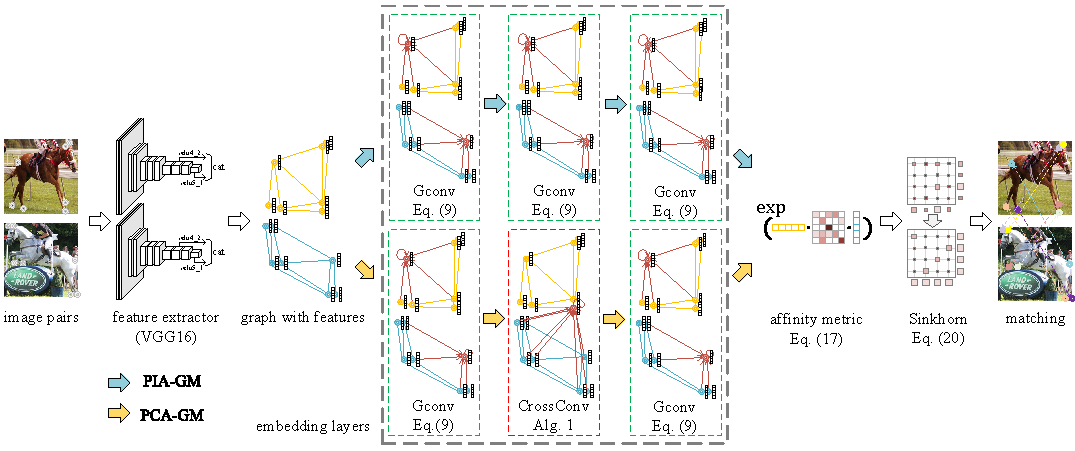
\includegraphics[width=0.85\linewidth]{Images/pia-pca.pdf}}

    \subfigure[IPCA-GM.]{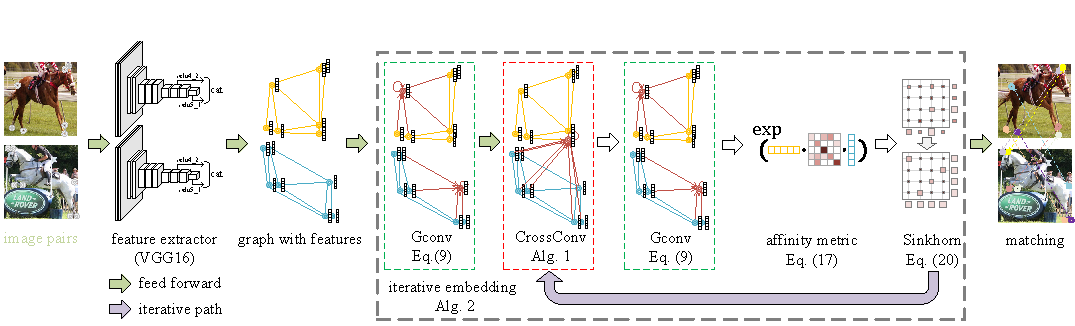
\includegraphics[width=0.85\linewidth]{Images/ipca.pdf}}

    \caption{Overview of methods proposed in \cite{pca-ipca}: PIA-GM, PCA-GM, and IPCA-GM. Pictures adopted from \cite{pca-ipca}.}
\end{figure}

\subsection{PIA-GM}
\textbf{P}ermutation loss and \textbf{i}ntra-graph \textbf{a}ffinity based \textbf{g}raph \textbf{m}atching (PIA-GM) proposed in \cite{pca-ipca} is the first method to adopt deep graph networks to compress a graph into node feature vectors. And they are then able to for the first time introduce the Sinkhorn \cite{sinkhorn} based permutation loss to solve the graph matching problem.

To be specific, PIA-GM first uses a graph embedding network to compress features around into each node. Then, the node feature vectors $\set{\mathbf{h}_{si}}$ are fed into an affinity network to obtain a node-wise affinity matrix $\mathbf{M}$. Next, Sinkhorn layer is used to convert the affinity matrix into a soft assignment in the form of a doubly-stochastic matrix $\mathbf{S}$. Finally, the permutation loss is applied to optimize the node correspondences. For final binary permutation matrix $\mathbf{X}$, we can perform Hungarian \cite{hungarian} algorithm on $\mathbf{S}$ as a final discretization step.

\textbf{Intra-graph node embedding.}
The intra-graph node embedding procedure fuses structural information into nodes so as to obtain $\set{\mathbf{h}_{si}}$ from $\set{\mathbf{h}_{si}^{(0)}}$. This is also called graph convolution (GConv). We apply GConv several times for gradually global information aggregation. One GConv step is defined as follows:

\begin{align}
    \mathbf{m}_{si}^{(k)} &= \frac{1}{\left|(i,j) \in \mathcal{E}_s\right|} \sum_{j: (i,j) \in \mathcal{E}_s} f_{\mathrm{msg}}\left(\mathbf{h}_{si}^{(k-1)}\right)\\
    \mathbf{n}_{si}^{(k)} &= f_{\mathrm{node}}\left( \mathbf{h}_{si}^{(k-1)} \right)\\
    \mathbf{h}_{si}^{(k)} &= f_{\mathrm{update}}\left( \mathbf{m}_{si}^{(k)}, \mathbf{n}_{si}^{(k)} \right)
\end{align}
where $\mathcal{E}_s$ is the set of edges in $s$-th graph, $f_{\mathrm{msg}}$, $f_{\mathrm{node}}$, and $f_{\mathrm{update}}$ are the message passing function, the self-passing function, and the update function, respectively. 
During the steps, $\mathbf{m}_{si}$ aggregates messages from neighbors of node $i$ and $\mathbf{n}_{si}$ processes the current node feature, then they are combined to update the node feature $\mathbf{h}_{si}$. 

\textbf{Affinity network.}
With all node features at hand, we need an affinity matrix $\mathbf{M}$ to describe node-to-node similarity between two graphs:
$$
\mathbf{M}_{ij} = f_{\mathrm{aff}}\left(\mathbf{h}_{1i}, \mathbf{h}_{2j}\right), \quad i\in \mathcal{V}_1, j\in \mathcal{V}_2
$$
where $f_{\mathrm{aff}}$ is the affinity score function, which is a weighted bi-linear function followed by an exponential function 
$$
f_{\mathrm{aff}}\left(\mathbf{h}_{1i}, \mathbf{h}_{2j} \right) = \exp\left(\frac{ \mathbf{h}_{1j}^\top \mathbf{K}  \mathbf{h}_{2j}}{\tau}\right)
$$
where $\mathbf{K}$ is the learnable weight, $\tau$ is the hyperparameter of temperature. for $\tau > 0$, with $\tau \rightarrow 0^+$, $f_{\mathrm{aff}}$ becomes more discriminative, while the chance of explosive gradient climbs.

\textbf{Sinkhorn layer.}
Sinkhorn \cite{sinkhorn} method is used as a relaxed approximation of Hungarian algorithm \cite{hungarian} for LAPs. It takes in any non-negative square matrix and outputs a doubly-stochastic matrix as prediction. The Sinkhorn operator is
\begin{align}
    \mathbf{M}'^{(k)} &=\mathbf{M}^{(k-1)} \oslash \left(\mathbf{M}^{(k-1)}\mathbf{1}\mathbf{1}^\top\right)\\
    \mathbf{M}^{(k)} &=\mathbf{M}'^{(k)} \oslash \left(\mathbf{1}\mathbf{1}^\top\mathbf{M}'^{(k)}\right)\\
\end{align}
where $\oslash$ means element-wise division, and $\mathbf{1}$ is an all-one column vector. In other word, Sinkhorn algorithm alternately takes row-normalization and column-normalization till convergence. For two graphs with different numbers of nodes, we can pad with some isolated dummy nodes.

With the doubly-stochastic prediction, it is natural to utilize cross-entropy loss as the objective, which is called "permutation" loss in \cite{pca-ipca}:
$$
\mathcal{L}_{\mathrm{CE}} = -\sum_{i\in \mathcal{V}_1, j\in \mathcal{V}_2 } \left(\mathbf{X}_{ij}^{\mathrm{gt}} \log\mathbf{S}_{ij} + \left(1-\mathbf{X}_{ij}^{\mathrm{gt}}\right) \log \left(1- \mathbf{S}_{ij}\right) \right)
$$

\subsection{PCA-GM}
As is proposed in \cite{pca-ipca}, \textbf{p}ermutation loss and \textbf{c}ross-graph \textbf{a}ffinity based \textbf{g}raph \textbf{m}atching (PCA-GM) is an improvement from PIA-GM. It introduces cross-graph fusion to boost cross-graph similarity discovery. For node $\mathbf{h}_{1i}$ in the first graph, the new cross-graph node embedding procedure (CrossConv) is defined as follows:
\begin{align}
    \mathbf{m}_{1i}^{(k)} &= \sum_{j\in \mathcal{V}_2} \hat{\mathbf{S}}_{i,j} f_{\mathrm{msg-cross}}\left(\mathbf{h}_{2j}^{(k-1)}\right)\\
    \mathbf{n}_{1i}^{(k)} &= f_{\mathrm{node-cross}}\left( \mathbf{h}_{1i}^{(k-1)} \right)\\
    \mathbf{h}_{1i}^{(k)} &= f_{\mathrm{update-cross}}\left( \mathbf{m}_{1i}^{(k)}, \mathbf{n}_{1i}^{(k)} \right)
\end{align}
where the node-to-node similarity $\hat{\mathbf{S}}$ is the doubly-stochastic matrix predicted from $\set{\mathbf{h}_{si}^{(k-1)}}$ with the affinity followed by the Sinkhorn layer.

\subsection{IPCA-GM}
Note that PCA-GM gets a pre-result $\hat{\mathbf{S}}$ for cross-graph aggregation. Then the final result $\mathbf{S}$ can be interpreted as a refinement of $\hat{\mathbf{S}}$. So, it is natural to perform this refinement iteratively, which is the main idea of \textbf{i}terative \textbf{p}ermutation loss and \textbf{c}ross-graph \textbf{a}ffinity based \textbf{g}raph \textbf{m}atching (IPCA-GM) \cite{pca-ipca}. The iterative refinement procedure is to do GConv and CrossConv alternately. Note that $\hat{\mathbf{S}}$ is calculated at the end of each CrossConv, GConv pair rather than before each CrossConv, which means the very first CrossConv is a "GConv" with different parameters.

\begin{figure}[htbp]
    \centering
    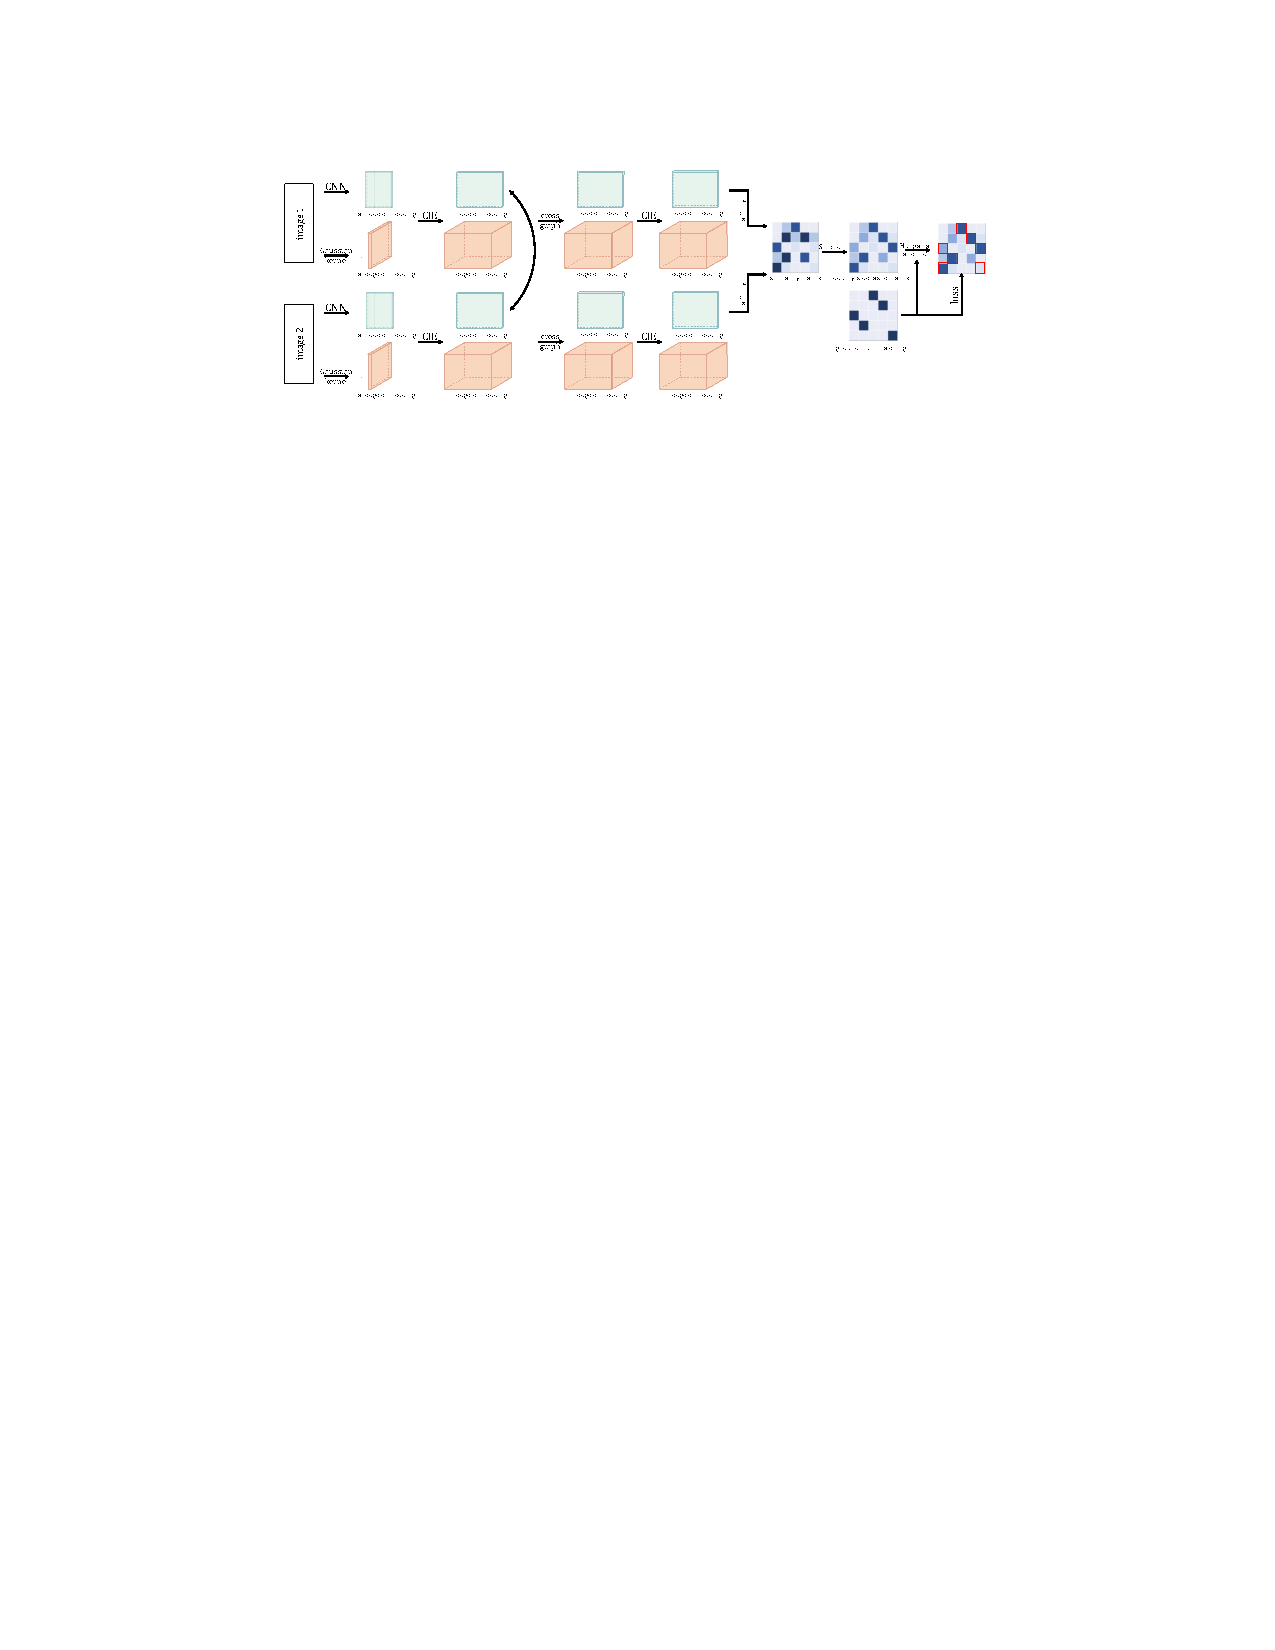
\includegraphics[width=0.85\linewidth]{Images/cie.pdf}
    \caption{Overall architecture proposed in \cite{cie}, consisting of channel-independent embedding and Hungarian attention. Picture adopted from \cite{cie}.}
\end{figure}
\subsection{CIE}



In all methods above, while structural features are perserved, edge attributes are neglected. \textbf{C}hannel-\textbf{I}ndependent \textbf{E}mbedding (CIE) \cite{cie} is then proposed to introduce edge attributes to LAPGM method. 

Taking edge embeddings $\set{\mathbf{e}_{sij}}$ into account, the new GNN method updates both node and edge embeddings simultaneously:
$$
\set{\mathbf{h}_{si}^{(k)}}  = f\left(\set{\mathbf{h}_{si}^{(k-1)}}, \set{\mathbf{e}_{sij}^{(k-1)}}, \mathbf{A}\right), \quad \set{\mathbf{e}_{sij}^{(k)}}  = g\left(\set{\mathbf{h}_{si}^{(k-1)}}, \set{\mathbf{e}_{sij}^{(k-1)}}, \mathbf{A}\right)
$$
where $\mathbf{A}$ is the adjacency matrix.


\begin{figure}[htbp]
    \centering
    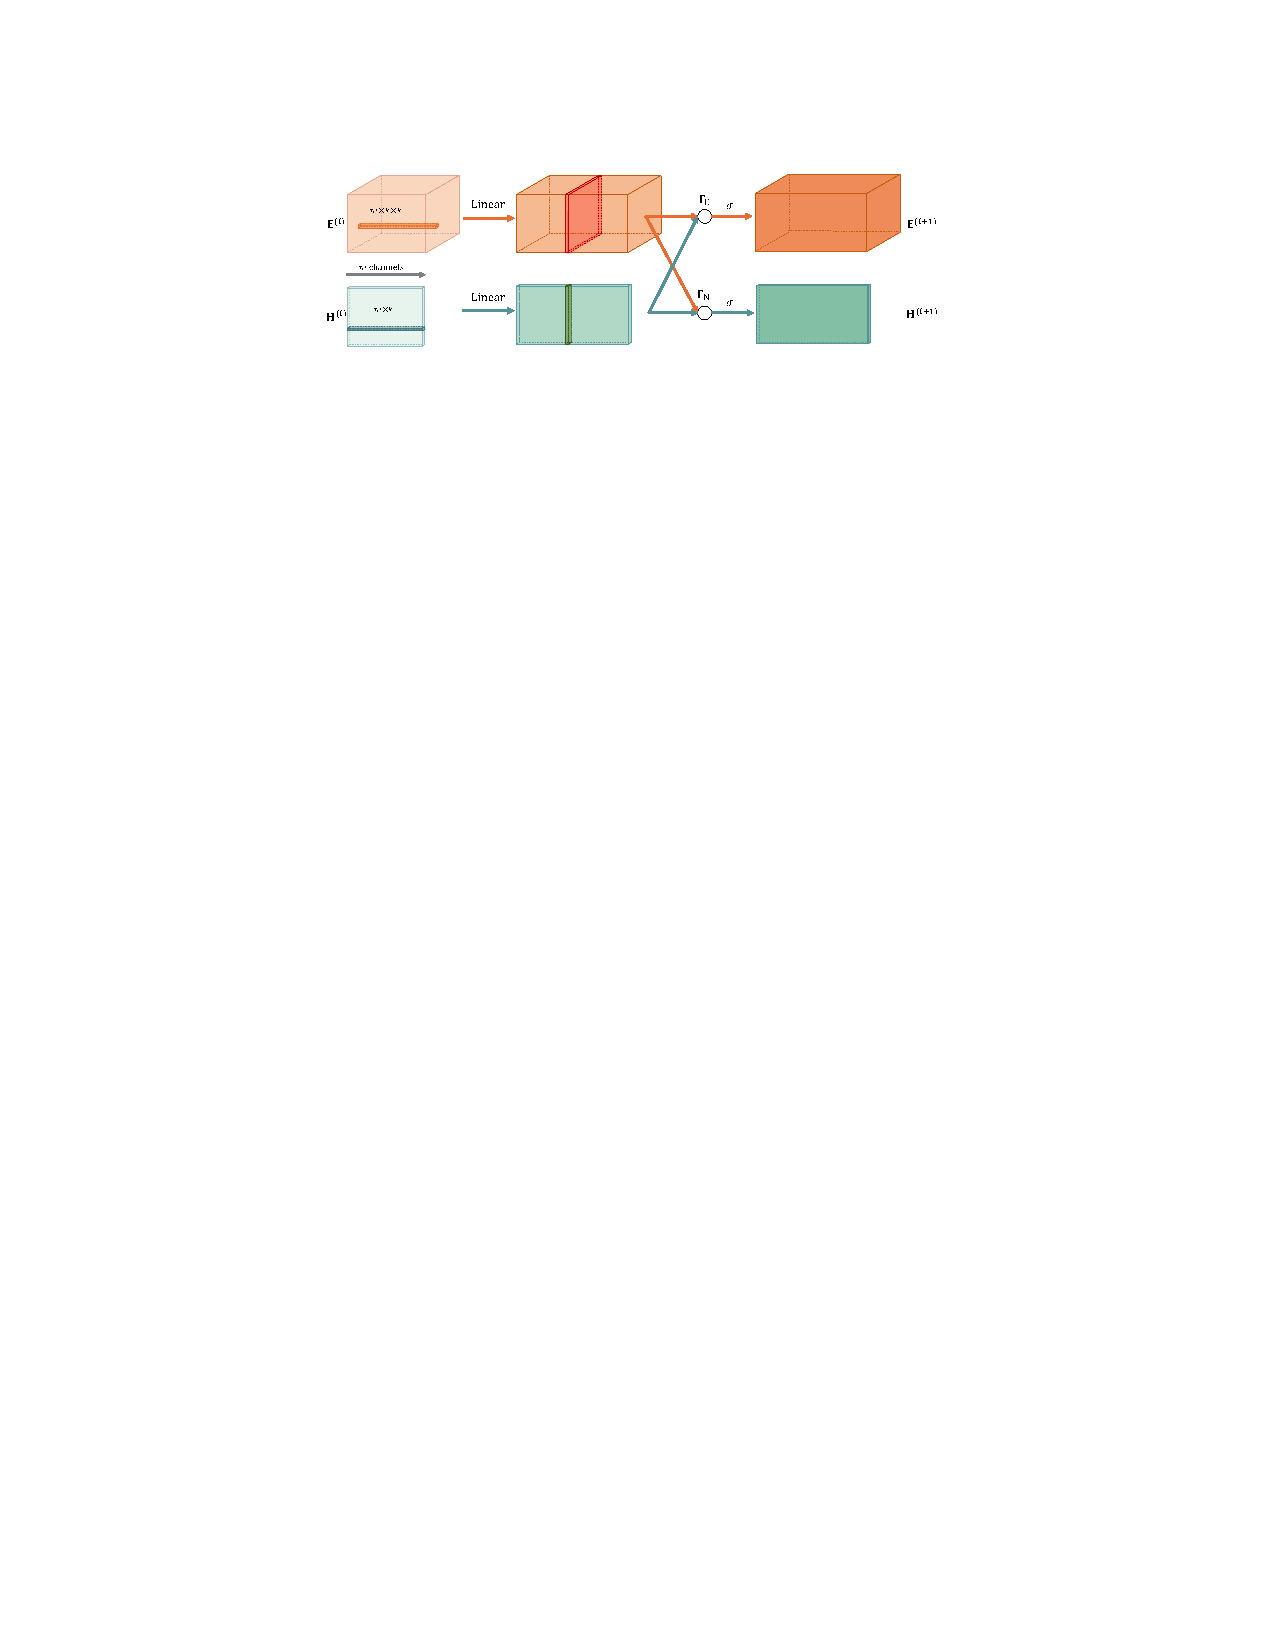
\includegraphics[width=0.6\linewidth]{Images/cie-detail.pdf}
    \caption{Channel-independent embedding. Picture adopted from \cite{cie}.}
\end{figure}

\textbf{Channel-Independent Embedding.}
As is stated in \cite{cie}, the representation ability of staightforward edge-wise merging is limited. Furthermore, fully connected merging is costy and causes instability for back-propagation. \textbf{C}hannel-\textbf{I}ndependent \textbf{E}mbedding (CIE) is proposed to merge embeddings in a channel-wise fashion
\begin{align}
    \mathbf{h}_{si}^{(k)} &= \sigma\left(\sum_{j:(i,j)\in \mathcal{E}_s} \Gamma_N \left(f_{\mathrm{msg-edge}}\left(\mathbf{e}_{sij}^{(k-1)}\right)  \circ f_{\mathrm{msg-node}}\left(\mathbf{h}_{sj}^{(k-1)}\right) \right) + \sigma\left(f_{\mathrm{node}\left(\mathbf{h}_{si}^{(k-1)}\right)}\right) \right)   \\
    \mathbf{e}_{sij}^{(k)} &= \sigma\left(\Gamma_E \left(f_{\mathrm{msg-edge}}\left(\mathbf{e}_{sij}^{(k-1)}\right)  \circ f_{\mathrm{msg-end}}\left(\mathbf{h}_{si}^{(k-1)}, \mathbf{h}_{sj}^{(k-1)}\right) \right) + \sigma\left(f_{\mathrm{msg-edge}\left(\mathbf{e}_{sij}^{(k-1)}\right)}\right) \right)  
\end{align}
where $\Gamma_N \left(\cdot \circ \cdot\right)$, $\Gamma_E \left(\cdot \circ \cdot\right)$ are channel-wise operators/functions, and $f_{\mathrm{msg-end}}(\cdot, \cdot)$ is commutative (for undirected graphs). Note that the cross-graph convolution step is still limited in node embeddings. It is also possible to extend the idea for edge embeddings, which require "affinity" values for every edge pair. What keeping us off is the significant computation demand. Here we again stress the "compressibility" of node embeddings for graphs.


\begin{figure}[htbp]
    \centering
    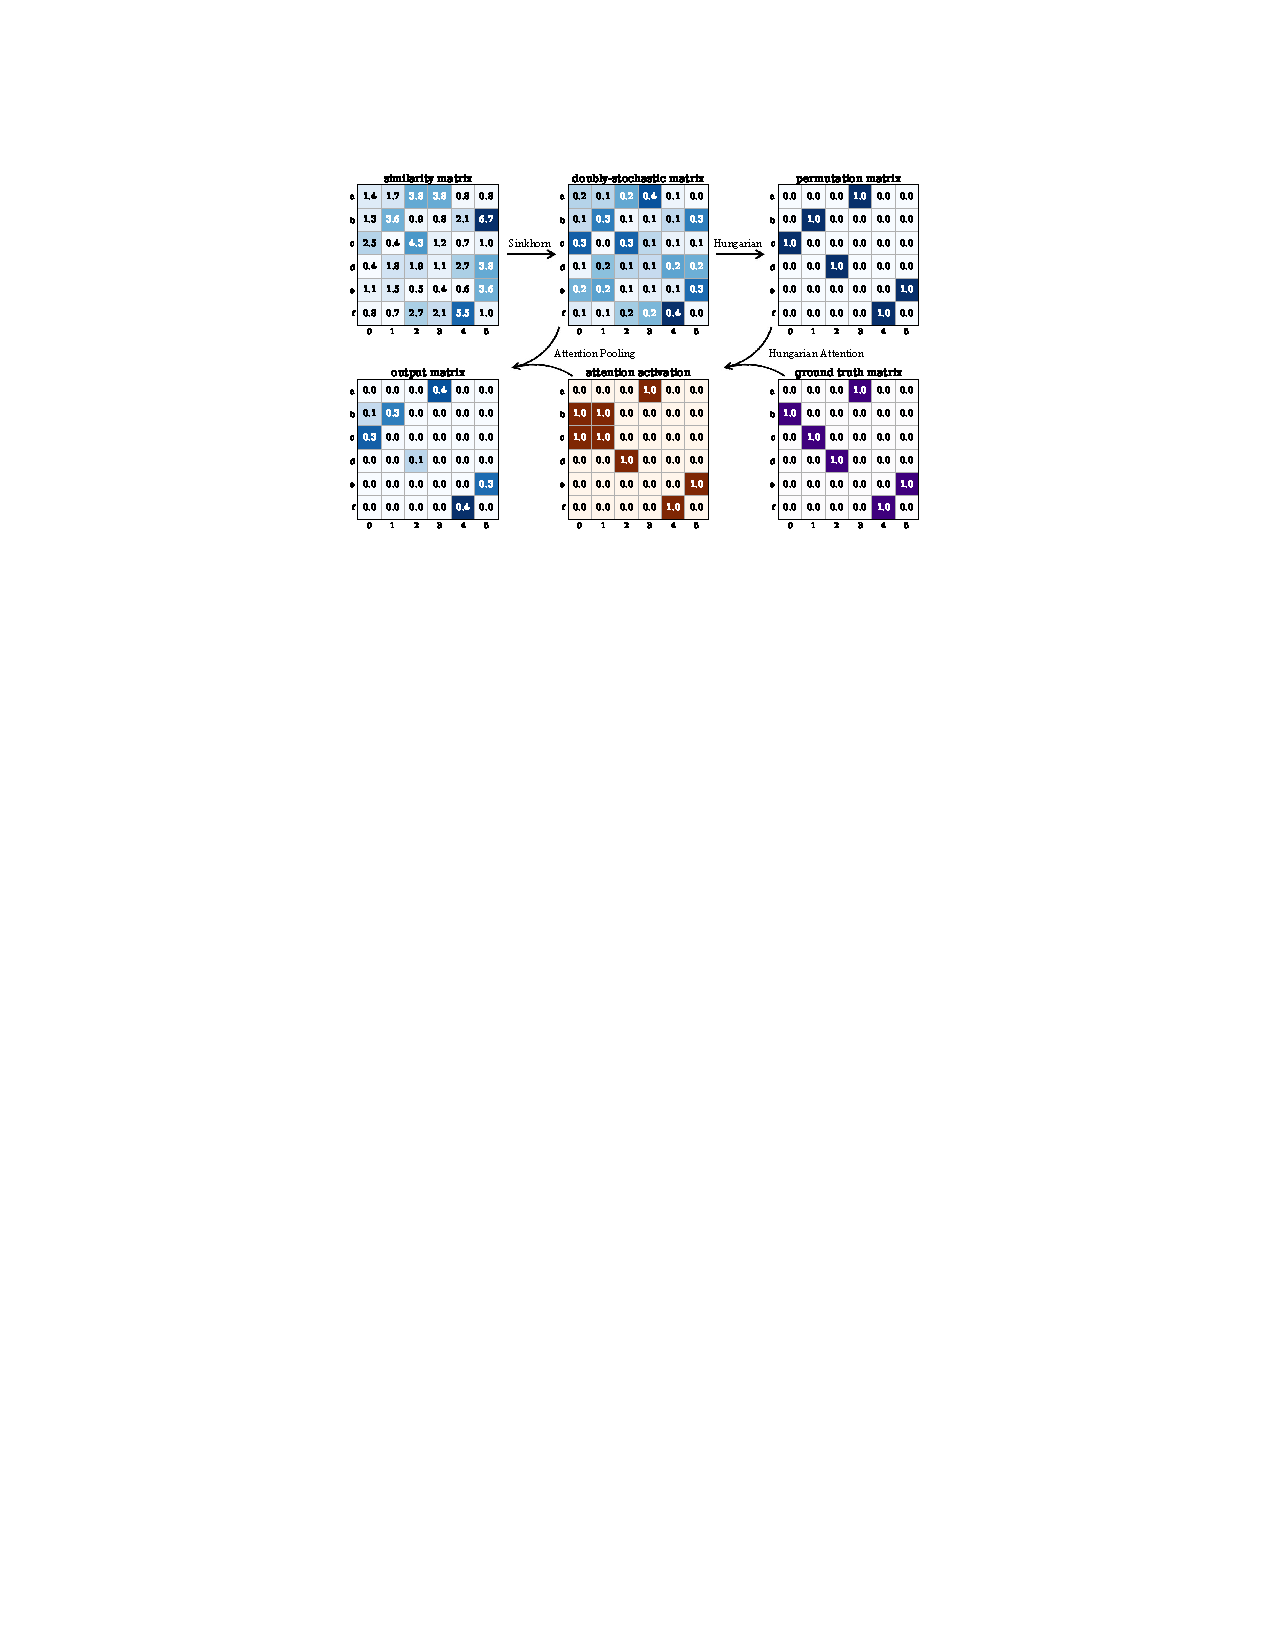
\includegraphics[width=0.5\linewidth]{Images/hungarian.pdf}
    \caption{Hungarian attention. Picture adopted from \cite{cie}.}
\end{figure}
\textbf{Hungarian attention.}
Cross-entropy loss prefers samples that are easy to learn in the early training stage and tends to perserve almost binary predictions (\cite{cie}). \cite{cie} proposed an improved attention mechanism to better back-propagation and have more unified training and testing interests (we used to train on continuous while test on discrete). They introduce a sparse attention mask as 
$$
\mathbf{Z} = \mathrm{Atten} \left(\mathbf{X}, \mathbf{X}^{\mathrm{gt}}\right)
$$
which is implemented as the union of output binary mask $\mathbf{X}$ and the ground-truth binary mask $\mathbf{X}^{\mathrm{gt}}$. The mask covers all points except for true negatives. They are trivial for optimization especially when we use Sinkhorn (or in other tasks, Softmax) to normalize the outputs. With Hungarian attention, the model is supposed to focus on the performance at ground truth matching and the digits that hinder the matching most. The Hungarian attention loss is defined as 
$$
\mathcal{H}_{\mathrm{CE}} = -\sum_{i\in \mathcal{V}_1, j\in \mathcal{V}_2 } \mathbf{Z}_{ij} \left(\mathbf{X}_{ij}^{\mathrm{gt}} \log\mathbf{S}_{ij} + \left(1-\mathbf{X}_{ij}^{\mathrm{gt}}\right) \log \left(1- \mathbf{S}_{ij}\right) \right)
$$

\textbf{Soft hungarian attention.} From our observation, the Hungarian attention loss does not improve performance every time. We suspect that the Hungarian attention loss is too strong to be used in the early training stage. The hard attention mechanism makes predictions noisy with submaximums. We thus propose a soft version of Hungarian attention loss, which depress loss from the wide true negatives up to a weight $\lambda_{\mathrm{H}}$. It is defined as
$$
\mathcal{H}_{\mathrm{CE}}^\mathrm{S} = -\sum_{i\in \mathcal{V}_1, j\in \mathcal{V}_2 } \left(\mathbf{Z}_{ij} + \lambda_{\mathrm{H}} \sim \mathbf{Z}_{ij}\right) \left(\mathbf{X}_{ij}^{\mathrm{gt}} \log\mathbf{S}_{ij} + \left(1-\mathbf{X}_{ij}^{\mathrm{gt}}\right) \log \left(1- \mathbf{S}_{ij}\right) \right)
$$
where $\sim$ is the bitwise NOT operator. Though formulated from totally different aspect, the soft Hungarian attention loss is computationally equivalent to a weighted sum of the original cross-entropy loss and Hungarian attention loss.

\section{Experiments}
We have done various experiments to compare the mentioned methods, to verify components, and to search for good hyperparameters. 

\subsection{Dataset}
We follow tutorials from Pygmtools \cite{pygmtools} to take WillowObject \cite{willow} as our main dataset. WillowObject is a dataset of images annotated with keypoints. There are altogether $5$ classes of images, winebottle, car, motorbike, duck, and face. As is shown in Table \ref{tab:compare}, face is the easiest class while duck is especially challenging. For fear of overfitting, the train-test set split is conventional so that each class has a balanced number of instances in the train set, resulting in a test set much larger than the train one. And to make up the inbalance of the test set, the overall mean accuracy is calcualted at the level of classes rather than instances.

\subsection{Methods Comparison}
We conduct experiments on PCA-GM, IPCA-GM, CIE, and their combination with Hungarian attention loss (i.e., CIE-H). In Table \ref{tab:compare}, we report their performance on WillowObject. Among all methods, CIE has the best performance. Despite more refinement steps, IPCA-GM does not beat PCA-GM, which may be caused by longer back-propagation paths.

\begin{table}[htbp]
    \centering
    \begin{tabular}{lcccccc}
        \toprule
        Method& Winebottle& Car& Motorbike& Duck& Face& Mean\\
        \midrule
        PCA-GM-w/oFT& $89.32\%$& $86.47\%$& $91.26\%$& $86.32\%$& $99.92\%$& $90.66\%$\\
        PCA-GM& $93.90\%$& $89.89\%$& $94.47\%$& $91.68\%$& $\mathbf{100.00\%}$& $93.99\%$\\
        PCA-GM-H& $92.62\%$& $89.42\%$& $90.74\%$& $91.68\%$& $\mathbf{100.00\%}$& $92.89\%$\\
        IPCA-GM& $\mathbf{95.35\%}$& $90.32\%$& $91.05\%$& $87.03\%$& $99.97\%$&$92.74\%$ \\
        IPCA-GM-H& $93.19\%$& $88.00\%$& $90.79\%$& $85.24\%$& $99.91\%$& $91.43\%$\\
        CIE& $93.65\%$& $\mathbf{95.58\%}$& $\mathbf{95.53\%}$& $\mathbf{92.80\%}$& $99.17\%$& $\mathbf{95.34\%}$\\
        CIE-H& $90.39\%$& $91.05\%$& $94.95\%$& $88.21\%$& $99.93\%$& $92.90\%$\\
        \bottomrule
    \end{tabular}
    \caption{Test accuracies of different methods on WillowObject dataset. -w/oFT means the method freezes the pretrained backbone without finetuning, -H means Hungarian attention.}
    \label{tab:compare}
\end{table}

\subsection{Ablation Study}
\textbf{Backbone finetuning.}
We use pretrained 2D convolutional backbone (VGG16 \cite{vgg}) for feature extraction. Then it is a natural question whether to further finetune the backbone while training the LAPGM model. In Table \ref{tab:compare} we see an overall performance gain with finetuing. So, LAPGM methods would benefit from finetuning learnable feature extractors in an end-to-end style.

\textbf{Edge embeddings.} 
We also see PCA-GM as a variant of CIE with no edge embeddings. As is shown in Table \ref{tab:compare}, the edge embeddings significantly boost the performance of our LAPGM model, especially for objects with more rigid and templated structures, i.e., car and motorbike.

\textbf{Hungarian attention.}
Though is described to improve performance of all methods in \cite{cie}, Hungarian does not necessarily lead to better results in our experiments (see methods with and without -H in Table \ref{tab:compare}). We also dig deeper into soft Hungarian attention based on CIE. The results are reported in Table \ref{tab:hungarian}. Suprisingly, we find that the model learn easier classes (face) better with Hungarian attention, trading off performance on harder classes. And it remains to be seen whether this phenomenon is restricted to WillowObject.

\begin{table}[htbp]
    \centering
    \begin{tabular}{lcccccc}
        \toprule
        $\lambda_{\mathrm{H}}$& Winebottle& Car& Motorbike& Duck& Face& Mean\\
        \midrule
        $0\quad (\mathcal{L}_{\mathrm{CE}})$&$93.65\%$& $\mathbf{95.58\%}$& $95.53\%$& $\mathbf{92.80\%}$& $99.17\%$& $\mathbf{95.34\%}$\\
        $0.1$& $93.42\%$& $89.53\%$& $96.79\%$& $89.72\%$& $99.73\%$& $93.84\%$\\
        $0.3$& $93.00\%$& $91.47\%$& $95.47\%$& $90.69\%$& $99.77\%$& $94.08\%$\\
        $0.5$& $92.32\%$& $91.84\%$& $93.89\%$& $90.53\%$& $99.85\%$& $93.69\%$\\
        $0.7$& $90.82\%$& $88.73\%$& $\mathbf{96.05\%}$& $90.76\%$& $99.68\%$& $93.21\%$\\
        $0.9$& $\mathbf{94.56\%}$& $90.47\%$& $92.21\%$& $89.08\%$& $\mathbf{99.97\%}$& $93.26\%$\\
        $1\quad (\mathcal{H}_{\mathrm{CE}})$& $90.39\%$& $91.05\%$& $94.95\%$& $88.21\%$& $99.93\%$& $92.90\%$\\
        \bottomrule
        
    \end{tabular}
    \caption{Test accuracies of different level of soft Hungarian attention based on CIE.}
    \label{tab:hungarian}
\end{table}

\subsection{Hyperparameter Search}
\textbf{Weight decay.}
Since the test accuracies are obviously worse than train accuracies, there should be some overfitting issues. To prevent overfitting, we choose to impose some regulations on the parameters so as to make the model simple and robust, which is called weight decay. From results shown in Table \ref{tab:weightdecay}, we conclude that with proper weight decay (about $1e-2$), the robustness grows while the model capacity does not fall much.

\begin{table}[htbp]
    \centering
    \begin{tabular}{lcccccc}
        \toprule
        Weight Decay& Winebottle& Car& Motorbike& Duck& Face& Mean\\
        \midrule
        $0$& $92.37\%$& $87.26\%$& $94.67\%$& $90.53\%$& $99.92\%$& $92.95\%$\\
        $1e-4$& $93.11\%$& $89.42\%$& $91.38\%$& $87.98\%$& $\mathbf{100.00\%}$& $92.38\%$\\
        $5e-4$& $\mathbf{95.14\%}$& $89.26\%$& $93.16\%$& $91.01\%$& $99.98\%$& $93.71\%$\\
        $1e-3$& $91.21\%$& $88.58\%$& $\mathbf{98.21\%}$& $90.30\%$& $99.99\%$& $93.66\%$\\
        $5e-3$& $92.19\%$& $\mathbf{92.11\%}$& $93.47\%$& $\mathbf{91.84\%}$& $\mathbf{100.00\%}$& $93.92\%$\\
        $1e-2$& $93.90\%$& $89.89\%$& $94.47\%$& $91.68\%$& $\mathbf{100.00\%}$& $\mathbf{93.99\%}$\\
        $5e-2$& $91.17\%$& $90.05\%$& $91.74\%$& $86.57\%$& $99.99\%$& $91.74\%$\\
        $1e-1$& $92.78\%$& $91.37\%$& $94.37\%$& $89.82\%$& $99.97\%$& $93.66\%$\\
        \bottomrule
        
    \end{tabular}
    \caption{Test accuracies of PCA-GM model with weight decay.}
    \label{tab:weightdecay}
\end{table}

\textbf{Optimizer.}
We have experimented with both AdamW and SGD optimizers. As the results shown in Table \ref{tab:optimizer}, AdamW stably optimize the model to a way better minima than SGD. Chances are that the learning rate is too big for SGD to converge.

\begin{table}[htbp]
    \centering
    \begin{tabular}{lcccccc}
        \toprule
        Optimizer& Winebottle& Car& Motorbike& Duck& Face& Mean\\
        \midrule
        AdamW& $\textbf{93.90\%}$& $\textbf{89.89\%}$& $\textbf{94.47\%}$& $\textbf{91.68\%}$& $\textbf{100.00\%}$& $\textbf{93.99\%}$\\
        SGD& $36.09\%$& $34.21\%$& $50.05\%$& $37.89\%$& $85.80\%$& $48.81\%$\\
        \bottomrule
        
    \end{tabular}
    \caption{Test accuracies of PCA-GM model with different optimizers.}
    \label{tab:optimizer}
\end{table}

\textbf{Learning rate scheduler.}
Several learning rate schedulers are tried. From Table \ref{tab:scheduler}, we find that different learning rate schedulers have similar performances in our task.

\begin{table}[htbp]
    \centering
    \begin{tabular}{lcccccc}
        \toprule
        LR Scheduler& Winebottle& Car& Motorbike& Duck& Face& Mean\\
        \midrule
        None& $\textbf{89.52\%}$& $86.05\%$& $\textbf{92.58\%}$& $86.76\%$& $99.93\%$& $\textbf{90.97\%}$\\
        StepLR& $88.85\%$& $86.32\%$& $91.79\%$& $85.15\%$& $\textbf{99.95\%}$& $90.41\%$\\
        CosineAnnealing& $89.16\%$& $\textbf{87.68\%}$& $89.68\%$& $\textbf{87.40\%}$& $99.93\%$& $90.77\%$\\
        \bottomrule
        
    \end{tabular}
    \caption{Test accuracies of PCA-GM model with different learning rate schedulers.}
    \label{tab:scheduler}
\end{table}

\textbf{More details.}
For learning rate, several candidate values are tried at an early stage of the project. Since the performance is rather high and AdamW is not so sensitive to learning rate, a fixed value of $1e-4$ is finally picked for all experiments with no further tuning.



\section{Implementation and Feedbacks}

\subsection{Trainer}
We aim to create a trainer which is modular, robust, and visible. It shall work fine with LAPGM models from Pygmtools \cite{pygmtools}. Even more, users can migrate it to any other deep learning task (better with Jittor \cite{jittor}) painlessly.

\textbf{Modularity.}
For better reusability and customizability, we build the \texttt{Trainer} class in a rather modular way. We make every module quite replacable, including \texttt{model}, \texttt{optimizer}, \texttt{lr\_scheduler}, data loaders, benchmarks, and even per-batch task, per-epoch task, evaluation, etc.. For tidiness, we do not implement some functions as callable arguments, but they are also easy to substitute.

\textbf{Robustness.}
Our trainer is robust and automated. It would log in file the training and testing process and save checkpoints automatically. Besides the main model, all states including training progress can be fully recorded (up to the config) and automatically resumed. Users need not to worry about accidents during training.

\textbf{Visibility.}
The training process and all informations are printed in a human-friendly way. You can supervise the progress with ease. By the way, all training statics like loss and metrics are connected to TensorBoard \cite{tensorflow}, ready for investigating and further processing.

\subsection{Dataset}
The dataset is implemented based on \texttt{benchmark} class from Pygmtools \cite{pygmtools} and \texttt{Dataset} class from Jittor \cite{jittor}, with which data loading and preprocessing are easy. For better compatibility, we have implemented Delaunay triangulation with both SciPy \cite{scipy} and OpenCV \cite{opencv}. Furthermore, since \texttt{benchmark} shuffles the order of keypoints each time loading data, we adviced that the cached ground truth should be refreshed at each shuffle for coherence, which has been adopted in newer versions of Pygmtools. As an abstract, the dataset is iterable. At each iteration, a batch (\texttt{dict}) of data is provided.

\textbf{WillowObject.}
This dataset is quite standard. We can directly use the universal implementation to get it smoothly involved in training.

\textbf{PascalVOC.}
Numbers of keypoints varies from instance to instance in PascalVOC \cite{voc1,voc2}. So we specially provide batch support based on padding and support for cases in which keypoints are less than $3$. For batch support, we rewrite \texttt{collate\_batch} to make all shapes correct. To fit the interface of \texttt{Benchmark.eval}, we perform a matrix-to-list pipeline while testing. We have intended to perform some quantitative experiments on PascalVOC, but a CUDA error from Jittor \cite{jittor} was reported for a long period and the dataset itself is too big to do full experiments. Consequently, only a compatibility test is done, which shows that our pipeline works with the dataset. (P.S., as is mentioned in the presentation, it would be more user-friendly if the \texttt{voc2011\_pairs.npz} file is downloaded automatically together with the main data.) 

\subsection{Model}
We have integrated multiple mentioned methods in one universal \texttt{LAPGM} class. It has two main modules, a 2D backbone module called \texttt{extractor} and a group matching module consisting of \texttt{gm\_fn} and \texttt{gm\_model} based on interfaces provided by Pygmtools \cite{pygmtools}. The model first extract feature from images and construct a graph from keypoints and the corresponding features. Then it passes the data to the graph matching method to get predictions. Finally, it calculates the loss if target is provided.

\textbf{Efficiency.}
During data processing, we sucessfully replace all possible Python loop with efficient batched operations provided by Jittor \cite{jittor}, so as to shorten inference time.

\textbf{Hungarian attention.}
Although it might be straightforward to implement Hungarian attention by reimplementing the permutation loss, we choose to use gradient hook instead. On one hand, gradient hook is orthognal to the loss on which Hungarian attention is applied. We can clearly see the weight applied to each element and replace the loss function without reimplementation. On the other hand, we are able to make more meaningful comparisons on loss if needed since they are calculated with the same equation.

\section{Acknowledgements}
Thanks to Dr. Junchi Yan for lectures and advice. Thanks to TAs (especially Runzhong Wang) for advice, instructions, and updates on Pygmtools \cite{pygmtools}. Thanks to Wenhao Zhang for help with debugging.

\newpage 
\bibliographystyle{plain}
\bibliography{reference}

\end{document}